\documentclass[oneside, 11pt]{article}

\usepackage[T1]{fontenc}
\usepackage[utf8]{inputenc}
\usepackage[dutch]{babel}

\usepackage{fouriernc}
\usepackage[detect-all, load-configurations=binary,
            separate-uncertainty=true, per-mode=symbol,
            retain-explicit-plus, range-phrase={ tot }]{siunitx}

\usepackage{setspace}
\setstretch{1.2}

\setlength{\parskip}{\smallskipamount}
\setlength{\parindent}{0pt}

\usepackage{geometry}
\geometry{marginparwidth=0.5cm, verbose, a4paper, tmargin=3cm, bmargin=3cm, lmargin=2cm, rmargin=2cm}

\usepackage{float}

\usepackage[fleqn]{amsmath}
\numberwithin{equation}{section}
\numberwithin{figure}{section}

\usepackage{graphicx}
\graphicspath{{Figures/}}
\usepackage{subfig}

\usepackage{tikz}
\usetikzlibrary{plotmarks}

\usepackage{fancyhdr}
\pagestyle{fancy}
\fancyhf{}
\rhead{\thepage}
\renewcommand{\footrulewidth}{0pt}
\renewcommand{\headrulewidth}{0pt}

\usepackage{relsize}
\usepackage{xspace}
\usepackage{url}

\newcommand{\figref}[1]{Figuur~\ref{#1}}

\newcommand{\hisparc}{\textsmaller{HiSPARC}\xspace}
\newcommand{\kascade}{\textsmaller{KASCADE}\xspace}
\newcommand{\sapphire}{\textsmaller{SAPPHiRE}\xspace}
\newcommand{\jsparc}{\textsmaller{jSparc}\xspace}
\newcommand{\hdf}{\textsmaller{HDF5}\xspace}
\newcommand{\aires}{\textsmaller{AIRES}\xspace}
\newcommand{\csv}{\textsmaller{CSV}\xspace}
\newcommand{\python}{\textsmaller{PYTHON}\xspace}
\newcommand{\corsika}{\textsmaller{CORSIKA}\xspace}
\newcommand{\labview}{\textsmaller{LabVIEW}\xspace}
\newcommand{\daq}{\textsmaller{DAQ}\xspace}
\newcommand{\adc}{\textsmaller{ADC}\xspace}
\newcommand{\adcs}{\textsmaller{ADC}s\xspace}
\newcommand{\Adcs}{A\textsmaller{DC}s\xspace}
\newcommand{\hi}{\textsc{h i}\xspace}
\newcommand{\hii}{\textsc{h ii}\xspace}
\newcommand{\mip}{\textsmaller{MIP}\xspace}
\newcommand{\hisparcii}{\textsmaller{HiSPARC II}\xspace}
\newcommand{\hisparciii}{\textsmaller{HiSPARC III}\xspace}
\newcommand{\pmt}{\textsmaller{PMT}\xspace}
\newcommand{\pmts}{\textsmaller{PMT}s\xspace}

\DeclareSIUnit{\electronvolt}{\ensuremath{\mathrm{e\!\!\:V}}}

\DeclareSIUnit{\unitsigma}{\ensuremath{\sigma}}
\DeclareSIUnit{\mip}{\textsmaller{MIP}}
\DeclareSIUnit{\adc}{\textsmaller{ADC}}

\DeclareSIUnit{\gauss}{G}
\DeclareSIUnit{\parsec}{pc}
\DeclareSIUnit{\year}{yr}



\begin{document}

\title{Richting Reconstructie}
\author{C.G.N. van Veen} 
\date{}

\maketitle

\section{Introductie}

HiSPARC heeft verschillende meetstations op scholen in heel Nederland staan. 
Met deze meetstations kunnen Extensive Air Showers geanalyseerd worden.
De stations varieren in het aantal detectorplaten en de vorm waarin,
die platen zijn opgesteld. De meest gebruikte stations hebben vier of twee platen.
De vormen waarin de platen van de stations zijn opgesteld varieren van een driehoek,
rechthoek tot twee detectorplaten naast elkaar.

Met alle stations zijn EAS te meten, maar voor de bepaling van de richting van een EAS, zijn 
stations met vier detectorplaten handiger.
  


\section{Richting Reconstructie}

Een EAS wordt op aarde geregistreerd door detectorplaten in een \hisparc-station. 
Omdat de EAS niet bij elke detector tegelijk aankomt, is uit de tijdsverschillen 
te reconstrueren uit welke richting de shower is gekomen. 
Er zijn echter belangrijke verschillen tussen hoekreconstructie met een station met twee detectorplaten en een station met drie detectorplaten. 
Bij een station met twee platen is de hoekreconstructie wat beperkter dan bij een station met vier platen. In figuur \ref{fig:showerfront2} kun je zien dat het showerfront twee detectorplaten passeert en het signaal van de tweede plaat  een $\Delta$t later arriveert. 
Uit verschil tussen tussen de aankomsttijd tussen de twee platen en de aanname dat het showerfront met de lichtsnelheid beweegt,
 kan eenvoudig de hoek van het showerfront met de platen uitgerekend worden. De berekende hoek $\phi$ geeft echter geen uitsluitsel over de richting vanwaar de lawine kwam.
 Een hoek berekening met deze grootheden zorgt dat de richting $\phi$ van de lawine rotatie symmetrisch is om de s-as, zoals te zien is in figuur \ref{fig:showerfront3}, 
waar de shower, die eenzelfde hoek van inval heeft,  is getekend als van de shower van boven. 

\begin{figure}[H]
    \centering
    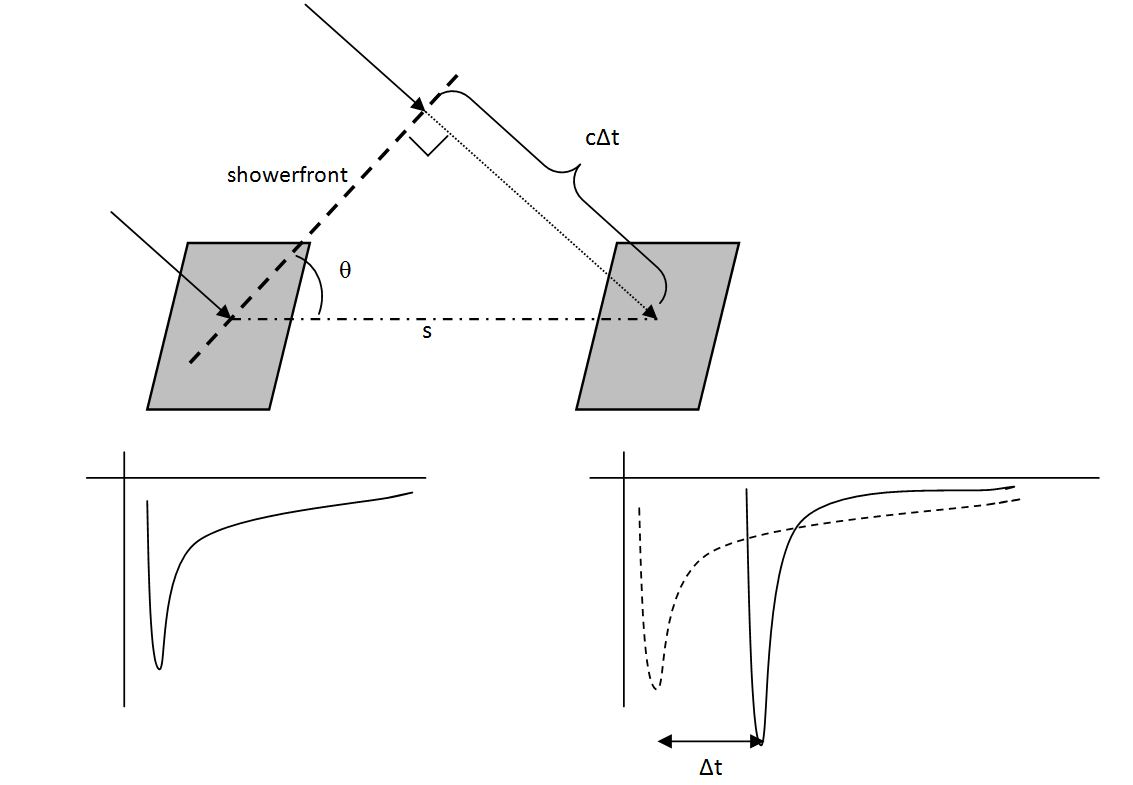
\includegraphics[scale=0.50]{showerfront2}
    \caption{Showerfront passeert de linker detector1. Een bepaalde tijd $\Delta$t later is het front bij de rechter detector. De shower reist met de lichtsnelheid en heeft dus schuin de afstand $c\Delta$t afgelegd.}
   \label{fig:showerfront2}
\end{figure}

\begin{figure}[H]
    \centering
    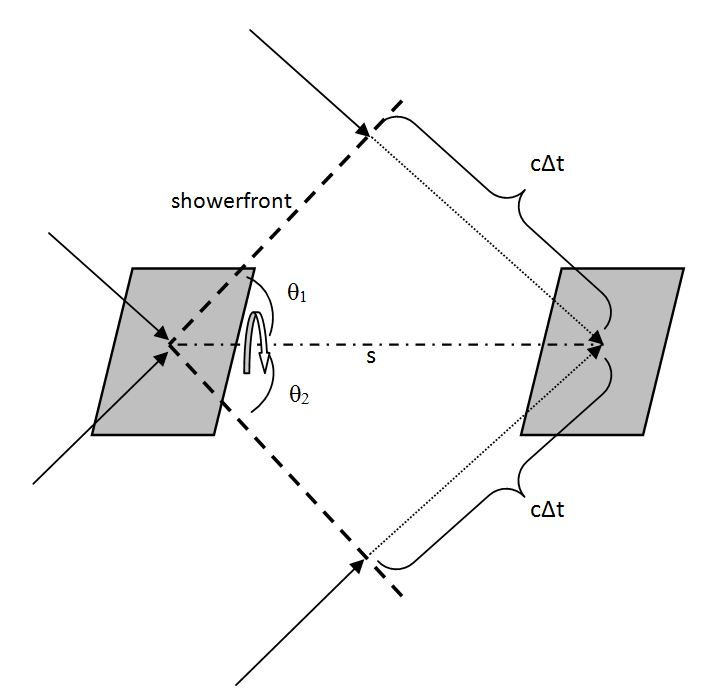
\includegraphics[scale=0.50]{showerfront3}
    \caption{Een shower vanuit richting $\phi t_{1}$ heeft dezelfde $c\Delta$t als een shower uit richting  $\phi t_{2}$. Met twee platen kun je de hoek vanwaar de shower komt dus niet bepalen. }
   \label{fig:showerfront3}
\end{figure}

Een hoekbepaling heeft dus minimaal drie detectoren nodig
In figuur \ref{fig:front} is een situatie weergegeven van een vlak showerfront
waarvan de normaal (de shower as) een zenithoek ($\theta$) heeft met het (x,y)-vlak en een azimuthoek($\phi$) met de x-as.

\begin{figure}[H]
    \centering
    %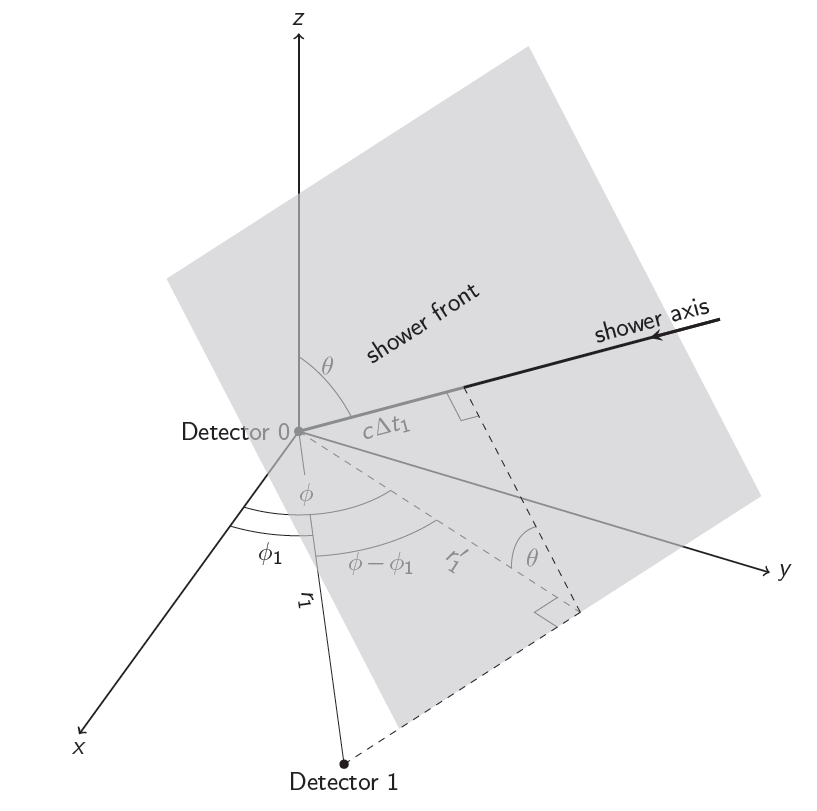
\includegraphics[scale=0.60]{front}
    \tdplotsetmaincoords{50}{115}
\pgfmathsetmacro{\axlen}{8}
\pgfmathsetmacro{\slen}{8}
\pgfmathsetmacro{\thetavec}{50}
\pgfmathsetmacro{\phivec}{70}
\pgfmathsetmacro{\phiovec}{30}
\pgfmathsetmacro{\rlen}{\slen * sin(\thetavec) / cos(\phivec - \phiovec)}
\pgfmathsetmacro{\splen}{\slen * sin(\thetavec) * sin(\thetavec)}
\pgfmathsetmacro{\ylen}{\slen * sin(\thetavec) * cos(\thetavec)}
\pgfmathsetmacro{\clen}{.5}

\begin{sansmath}
\begin{tikzpicture}[tdplot_main_coords, node distance=0pt, font=\sffamily]

% Set coordinates
\coordinate (O) at (0, 0, 0);
\tdplotsetcoord{S}{\slen}{\thetavec}{\phivec}
\tdplotsetcoord{D}{\rlen}{90}{\phiovec}
\tdplotsetcoord{S'}{\splen}{\thetavec}{\phivec}

% Draw axes
\draw[thick,->] (0, 0, 0) -- (\axlen, 0, 0) node[anchor=north]{$x$};
\draw[thick,->] (0, 0, 0) -- (0, \axlen, 0) node[anchor=west]{$y$};
\draw[thick,->] (0, 0, 0) -- (0, 0, \axlen) node[anchor=south]{$z$};

% Draw detector points
\fill (O) circle (2pt);
\node at (O) [anchor=east] {Detector 0};
\fill (D) circle (2pt);
\node at (D) [anchor=north] {Detector 1};

% Draw labelled lines
\draw[very thick] (O) -- (S');
\path (O) -- (S') node [midway,below,sloped] {$c \Delta t_1$};
\draw[dashed] (O) -- (Sxy) node [pos=.6,below,sloped] {$r'_1$};
\draw (O) -- (D) node [midway,below,sloped] {$r_1$};

% Draw phi angle arcs
\tdplotdrawarc{(O)}{2}{0}{\phivec}{above left,fill=white}{$\phi$}
\tdplotdrawarc{(O)}{2.5}{0}{\phiovec}{below}{$\phi_1$}
\tdplotdrawarc{(O)}{3}{\phiovec}{\phivec}{below}{$\phi - \phi_1$}

% Draw theta angle arcs and right angle square
\tdplotsetthetaplanecoords{\phivec}
\tdplotdrawarc[tdplot_rotated_coords]{(O)}{1.5}{0}{\thetavec}{above}{$\theta$}
\tdplotdrawarc[tdplot_rotated_coords]{(Sxy)}{1.5}{-90 + \thetavec}{-90}{below right}{$\theta$}

% Draw right angle square in rotated theta plane
\tdplotsetrotatedcoords{\phivec-90}{90}{90-\thetavec}
\draw[tdplot_rotated_coords] ($(S') + (\clen,0)$) -- +(0,-\clen) -- +(-\clen,-\clen);

% Draw right angle on ground
\tdplotsetrotatedcoords{\phivec-90}{0}{0}
\draw[tdplot_rotated_coords] ($(Sxy) + (\clen,0)$) -- +(0,-\clen) -- +(-\clen,-\clen);

% Draw shower front
\tdplotsetrotatedcoords{\phivec}{\thetavec}{0}
\fill[tdplot_rotated_coords,gray!50,opacity=.6] ($(S')-(\ylen,\ylen,0)$) -- +(2*\ylen,0,0) -- +(2*\ylen,2*\ylen,0) -- +(0,2*\ylen,0) -- cycle;
\path[tdplot_rotated_coords] ($(S')-(0,\ylen,0)$) -- +(0,2*\ylen,0) node [midway,sloped,above,inner sep=30] {shower front};

% Draw lines in front of shower front
\draw[very thick] (S') -- ($(S')!2.2!(S)$) node [near end,above,sloped] {shower axis};
\draw[very thick,-stealth] ($(S')!2.2!(S)$) -- ($(S')!1.6!(S)$);
\draw[dashed] (D) -- (Sxy);
\draw[dashed] (Sxy) -- (S');

\end{tikzpicture}
\end{sansmath}

    \caption{Showerfront passeert detector 1. Een bepaalde tijd $\Delta$t1 later is het front bij detector 0.  Figuur overgenomen uit  \cite{Fokkema}}\label{fig:front}
\end{figure}

Het front passeert detector 1. Een bepaalde tijd $\Delta t_{1}$ later is het front bij detector 0. Op een gelijke wijze kan ook een $\Delta t_{2}$ worden bepaald, het tijdsverschil tussen detector 0 en detector 2. Voor de hoekreconstructie zijn dus minimaal drie detectoren nodig. In de HiSPARC-opstelling zijn dit òf de drie buitenste detectorplaten in een station, òf drie stations in een stationscluster. Al eerder is een dergelijke hoekreconstructie uitgevoerd met de volgende vergelijkingen, afgeleid door D. Fokkema \cite{Fokkema}:

%check deze vergelijking op hoek grieks!!
\begin{equation}
	   \quad \tan(\phi)= \frac{r_1\Delta t_1\cos\phi_1-r_2\Delta t_2\cos \phi_2}{r_1\Delta t_1\sin\phi_1-r_2\Delta t_2\sin \phi_2}
\end{equation}

\begin{equation}
	    \quad \sin(\theta)= \frac{c\Delta t_1}{r_1\cos(\phi-\phi_1)}
\end{equation}

%($\mathbf{F}_{actie}=-\mathbf{F}_{reactie}$) 

Hierin is $\phi_{1}$ de hoek tussen detector 0 en detector 1 en $r_{1}$ de afstand tussen deze detectoren. $\phi_{2}$ is de hoek tussen detector 0 en detector 2 en $r_{2}$ de afstand tussen deze detectoren. $c$ is de lichtsnelheid.

%Voor en na de botsing is deze kracht 0N. Gedurende de botsing,
%die voor beide objecten even lang duurt, zijn er twee even grote en
%tegengestelde krachten. Als voorwerp I gedurende de botsing vertraagt,
%versnelt voorwerp II. We kunnen deze (eenparig) versnelde bewegingen dus
%nader bestuderen met de tweede wet van Newton:





\begin{equation}
    \mathbf{F}=m\mathbf{a}
\end{equation}

Meer tekst en na de botsing. Gedurende de botsing, die voor beide
objecten even lang duurt, zijn er twee even grote en tegengestelde
krachten. Als voorwerp I gedurende de botsing vertraagt, versnelt
voorwerp II. We kunnen deze (eenparig) versnelde bewegingen dus nader
bestuderen met de tweede wet van Newto.

%\begin{figure}[H]
%    \centering
%    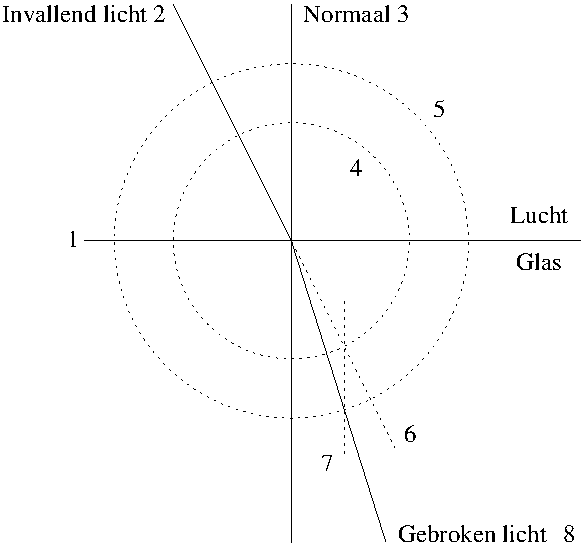
\includegraphics[scale=0.75]{vlak}
%    \caption{De breking aan een plat vlak}\label{fig:front}
%\end{figure}

Gedurende de botsing, die voor beide objecten even lang duurt, zijn er
twee even grote en \cite{klaasboekje} tegengestelde krachten. Als voorwerp I gedurende de
botsing vertraagt, versnelt voorwerp II.

\begin{thebibliography}{9}
    \bibitem{Fokkema}
        D.B.R.A. Fokkema, \emph{The \hisparc Experiment, data acquisition and reconstruction of shower direction}, PhD. thesis 2012
\end{thebibliography}

%\footnote{Ik gebruik voor
%de vector van de kracht "$\mathbf{F}$", de grootte wordt geschreven met
%"$F$".} oefenen beide objecten in het systeem op ieder moment een even
%grote maar tegengestelde kracht uit \footnote{Let op: Dit is een ander
%situatie dan een object waarbij alle krachten die op dat object werken
%in evenwicht zijn. Dit laatste is een bijzonder geval van de tweede wet
%Newton.}.

\end{document}
